\documentclass[portrait,a0,final]{a0poster}

\usepackage[utf8]{inputenc}
\usepackage[OT1]{fontenc}
\usepackage[french]{babel}
\usepackage{enumitem}
\usepackage{verbatim}
\usepackage{amsfonts, amsmath, amssymb, amsthm, dsfont}

%\usepackage{listings}
%\lstset{language=[Objective]Caml}

\usepackage{minted}

\usepackage{bussproofs}
\newcommand\typ[2]{\Gamma\vdash#1:#2}

\usepackage{multicol}
\usepackage[dvipsnames]{xcolor}
\usepackage{graphicx}
\usepackage{wrapfig}
\usepackage{tikz}

\usepackage[right=1cm,left=1cm,top=1cm,bottom=1cm]{geometry}
\setlength{\parindent}{0.0cm}
\renewcommand{\sfdefault}{lmss}

\definecolor{orangeinria}{RGB}{227,55,41} % Orange INRIA
\definecolor{color1}{RGB}{227,55,41} % Orange INRIA
\definecolor{color2}{RGB}{116,101,110} % Blue INRIA
\definecolor{orange}{RGB}{243,154,38}
\definecolor{red}{RGB}{226,0,38}
\definecolor{orange2}{RGB}{236,117,40}
\definecolor{grey}{RGB}{50, 50, 50}

% args: width, number, title, txt
\newcommand{\tblock}[2]{
%  \addtocounter{nblock}{1}
  \begin{tikzpicture}
    \tikzstyle{txtblock}=[draw=grey,rounded corners=40pt]
    \draw node (zou) [txtblock, text width=0.9 \columnwidth, inner sep=25pt, line width=5pt, text justified] {
	\Large #2
    };
    \draw node () at (zou.north) [line width=10pt,inner sep=15pt,anchor=center,fill=white] {
      \begin{Huge}
        \textcolor{orangeinria}{\textbf{#1}}
      \end{Huge}
    };
  \end{tikzpicture}
  \vspace{10mm}
}

\newcommand{\cblock}[2]{
%  \addtocounter{nblock}{1}
  \begin{tikzpicture}
    \tikzstyle{txtblock}=[draw=grey,rounded corners=40pt,fill=gray!10]
    \draw node (zou) [txtblock, text width=0.9 \columnwidth, inner sep=25pt, line width=5pt, text justified] {
	\Large #2
    };
    \draw node () at (zou.north) [line width=10pt,inner sep=15pt,anchor=center,fill=white] {
      \begin{Huge}
        \textcolor{orangeinria}{\textbf{#1}}
      \end{Huge}
    };
  \end{tikzpicture}
  \vspace{10mm}
}


\newcommand{\block}[1]{
%  \addtocounter{nblock}{1}
  \begin{tikzpicture}
    \tikzstyle{txtblock}=[draw=grey,fill=gray!10]
    \draw node (zou) [txtblock, text width=0.9 \columnwidth, inner sep=25pt, line width=4pt, text justified] {
      \Large #1
    };
  \end{tikzpicture}
  \vspace{10mm}
}

% args: title, authors, affiliation
\newcommand{\postertitle}[3]{
  \begin{tikzpicture}
    \draw node (titlebar) [inner sep=0cm, 
                           inner ysep=10mm,
                           text width=\textwidth, fill=orangeinria] {
        \hspace{0.2 \textwidth}
        \begin{minipage}[c]{0.79 \textwidth}
            \begin{center}
                \begin{VeryHuge}
                    {\color{white} \bfseries
                      #1
                    }
                \end{VeryHuge}
              \end{center}
            \end{minipage}
};

    \draw node (authors) at (titlebar.south) [anchor=north, yshift=-5mm,
                           text width=\textwidth, inner xsep=0cm] {
        \hspace{0.2 \textwidth}
        \begin{minipage}[c]{0.79 \textwidth}
            \begin{center}
                \begin{huge}
                  \color{orangeinria}
                  \textbf{#2}

                  \vspace{5mm}

                  #3
                \end{huge}
            \end{center}
        \end{minipage}
    };

    \node[xshift=0.1 \textwidth, yshift=-15mm] (logo) at (titlebar.west) {};

    \foreach \s in {0, 0.25, ..., 2.5}
    {
      \node[xshift=\s mm, yshift=-\s mm,fill=grey,opacity=0.07,rounded corners=20pt,line width=2pt, minimum width=0.18 \textwidth, minimum height=0.18 \textwidth] () at (logo) {
      };
    }

    \node[draw=grey,rounded corners=20pt,fill=white,line width=2pt, minimum width=0.18 \textwidth, minimum height=0.18 \textwidth] () at (logo) {
      
\includegraphics[width=0.16 \textwidth]{logo.jpg}
    };
\end{tikzpicture}
}


\def\aez{\textsf{Alt-Ergo~Zero}}
\def\altergo{\textsf{Alt-Ergo}}
\def\ens{\textsf{ENS Paris-Saclay}}
\def\inria{\textsf{Inria}}
\def\lsv{\textsf{LSV}}
\def\msat{\textsf{mSAT}}
\def\opam{\textsf{opam}}

\begin{document}

\sffamily % Font Family

\postertitle
{\msat{}:~An~OCaml~SAT~Solver}
{Guillaume \textsc{Bury}}
{DEDUC$\vdash$EAM (INRIA) - LSV / CNRS\\
\Large \textcolor{black}{\texttt{guillaume.bury@inria.fr}}}

\begin{center}

\begin{multicols}{2}

\tblock{Introduction} % TODO
{
  \vspace{0.5cm} % Pour pas se faire manger par le titre

  \msat{}: a SAT solving library in OCaml. It solves the \textbf{satisfibility}
  of propositional clauses. It is \textbf{Modular}: the user provides
  the theory. And it \textbf{produces formal proofs}.
}

\tblock{Conflict Driven Clause Learning}
{
  \begin{description}
    \item[Propagation] If there exists a clause $C = C' \lor a$, where
      $C'$ is false in the partial model, then add $a \mapsto \top$ to
      the partial model, and record $C$ as the reason for $a$.
    \item[Decision] Take an atom $a$ that is not yet in the partial model,
      and add $a \mapsto \top$ to the model.
    \item[Conflict] A conflict is a clause $C$ that is false in the current partial
      model.
    \item[Analyze] Perform resolution between the analyzed clause and the reason
      behind the propagation of its most recently assigned litteral, until
      the analyzed clause is suitable for backumping.
    \item[Backjump] A clause is suitable for backjumping if its most recently
      assigned litteral $a$ is a decision. We can then backtrack to before the
      decision, and add the analyzed clause to the solver, which will then enable
      to propagate $a \mapsto \bot$.
    \item[SMT] Formulas using first-order theories can be handled using a theory.
      Each formula propagated or decided is sent to the theory, which then
      has the duty to check whether the conjunction of all formulas seen so
      far is satisfiable, if not, it should return a theory tautology (as a clause),
      that is not satisfied in the current partial model.
  \end{description}
}

\tblock{Implementation}
{
  \begin{itemize}[label=$\blacktriangleright$]
    \item Imperative design
      \begin{itemize}[label=\checkmark]
        \item 2-watch litteral
        \item Backtrackable theories (less demanding than immutable theories)
      \end{itemize}
    \item Features
      \begin{itemize}[label=\checkmark]
        \item Functorized design, using generative functors
        \item Local assumptions
        \item Model output and proof output (Coq, dot)
      \end{itemize}
  \end{itemize}
}

\cblock{Solver Interface}
{
  \inputminted{ocaml}{solver_intf.ml}
}

\tblock{Other Solvers}
{
  \begin{center}
    \begin{tabular}{c@{\quad}|@{\quad}c@{\quad}|@{\quad}c@{\quad}|@{\quad}c}
    regstab & SAT & binary only & only pure SAT \\ \hline
    \begin{tabular}{c}\textbf{minisat}\\\textbf{sattools}\\ocaml-sat-solvers\end{tabular} & SAT & C bindings & only pure SAT \\ \hline
    Alt-ergo & SMT & binary only & Fixed theory \\ \hline
    \textbf{Alt-ergo-zero} & SMT & OCaml lib & Fixed theory \\ \hline
    \begin{tabular}{c}ocamlyices\\yices2\end{tabular} & SMT & C bindings & Fixed theory \\
  \end{tabular}
  \end{center}
}


\columnbreak

\tblock{Problem Example}
{
  \vspace{.2cm}
  \[
  \begin{matrix}
    \text{Are the following} & \quad & H1: & a = b   & \quad & H2: & b = c \lor b = d \\
    \text{hypotheses satisfible ?} & \quad & H3: & a <> d  & \quad & H4: & a <> c \\
  \end{matrix}
  \]
  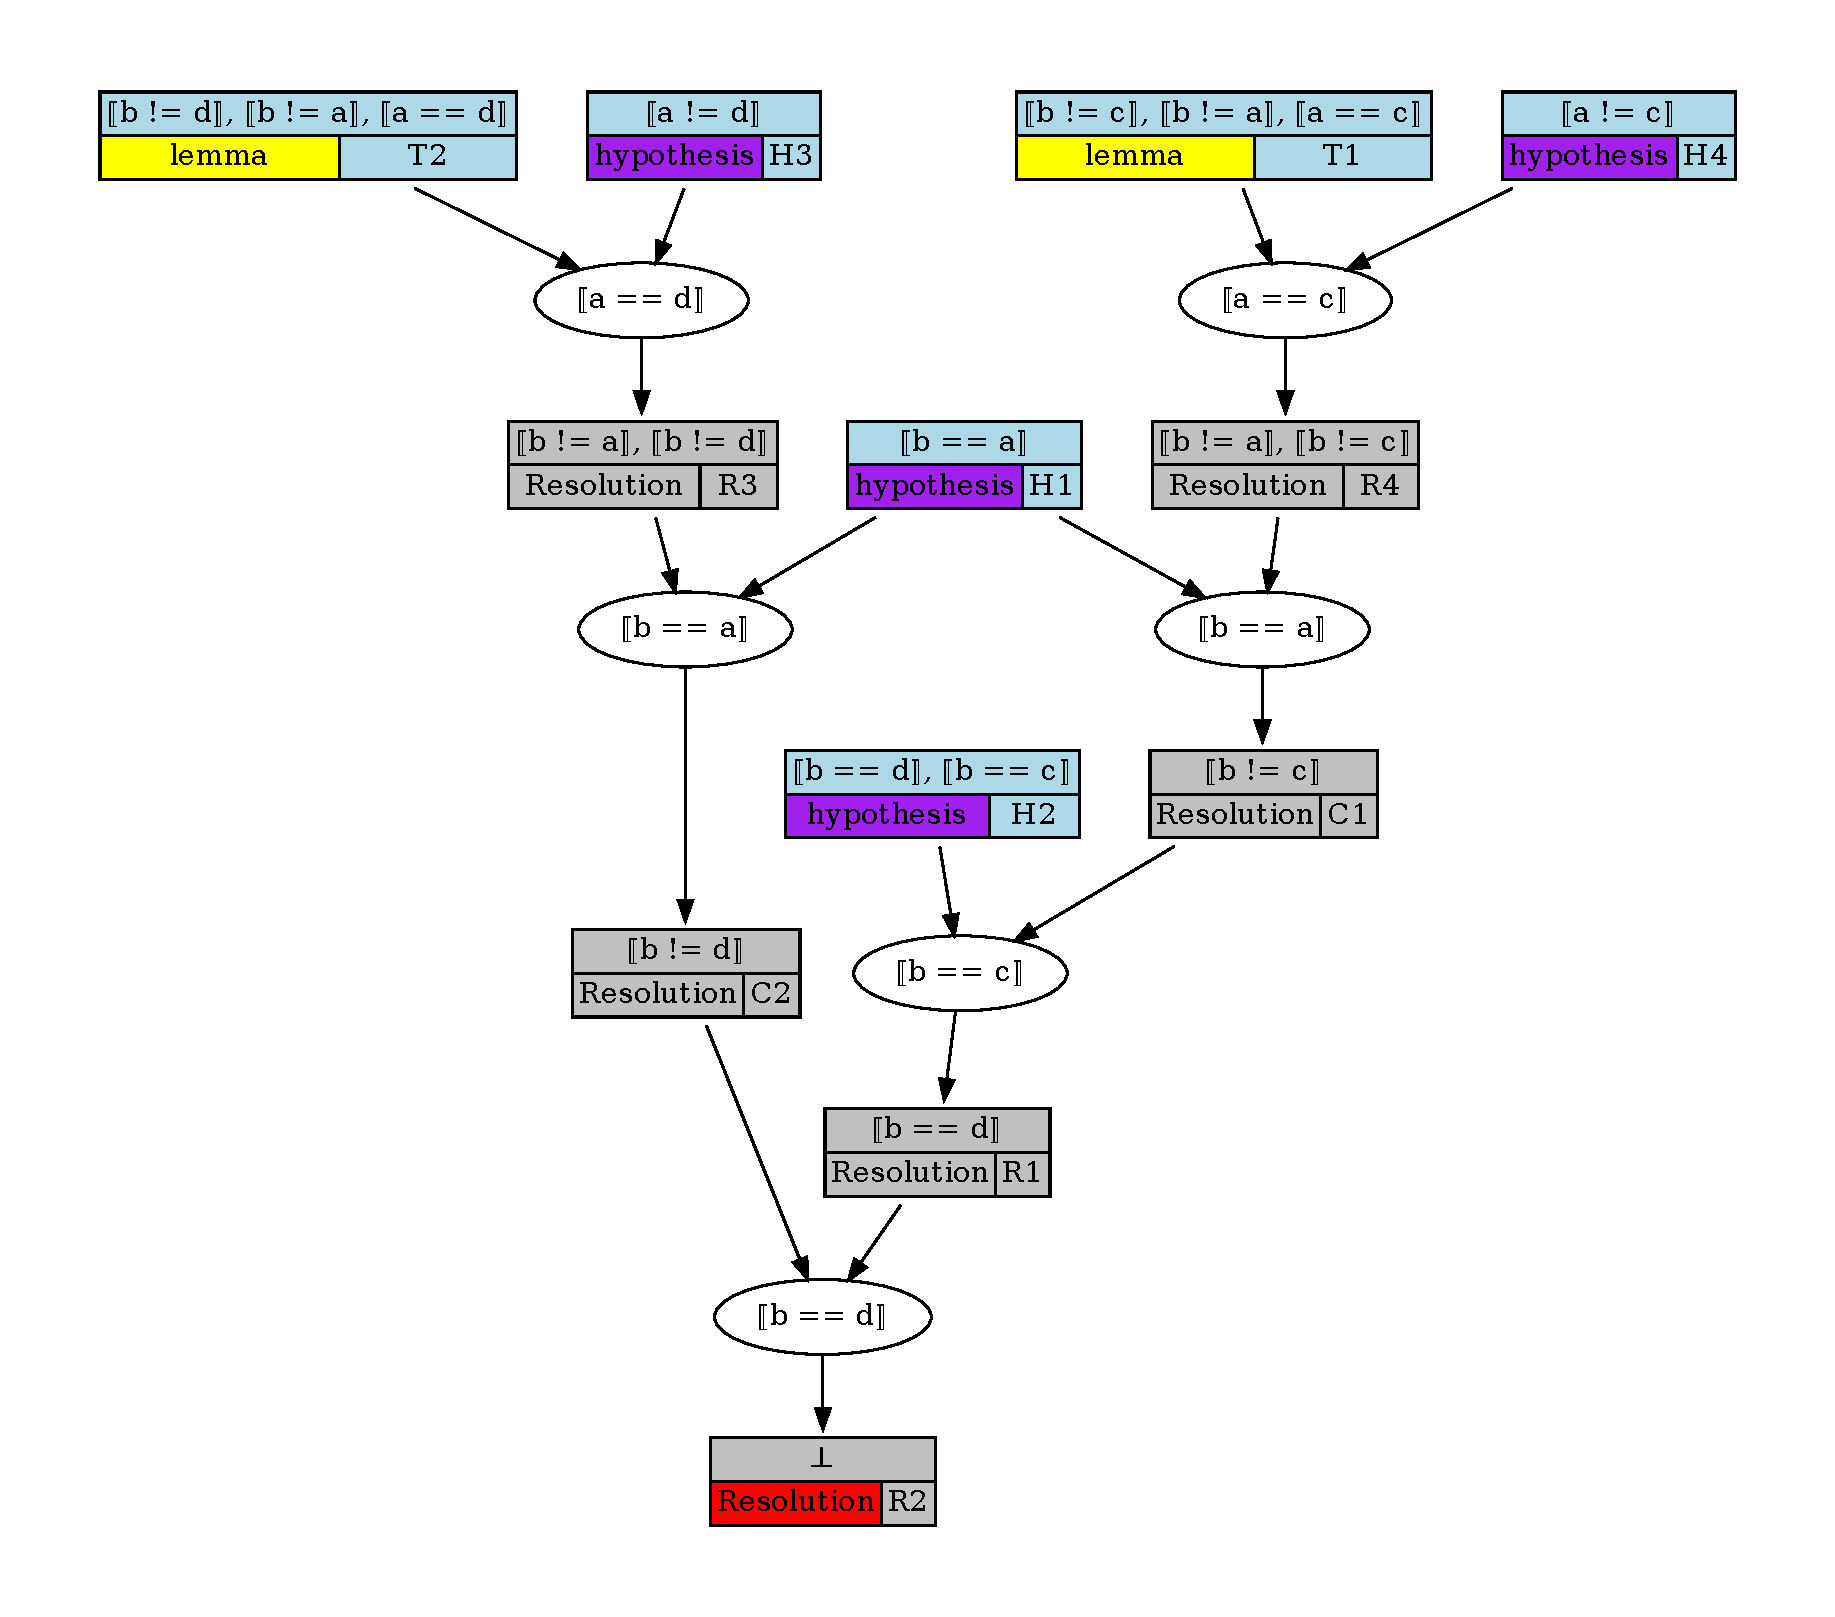
\includegraphics[height=33cm]{proof}
}

\cblock{Theory Interface}
{
  \inputminted{ocaml}{theory_intf.ml}
}

\tblock{Proof generation}
{
  \begin{itemize}[label=\checkmark]
    \item Each clause records its "history" which is the clauses
      used during analyzing
    \item Minimal impact on proof search (already done to compute
      unsat-core)
    \item Sufficient to rebuild the whole resolution tree
    \item A proof is a clause and proof nodes are expanded on demand\\
      $\rightarrow$ no memory issue
    \item Enables various proof outputs:
      \begin{itemize}[label=$\bullet$]
        \item Dot/Graphviz (see example above)
        \item Coq (and soon dedukti) formal proofs
      \end{itemize}
  \end{itemize}
}

\tblock{Performances}
{
  \\ \\
  \begin{tabular}{c|@{\,}c@{\,}|@{\,}c@{\,}|c|c}
    solvers & \begin{tabular}{c}Alt-ergo-zero\\{\small aez}\end{tabular} & \begin{tabular}{c}mSAT\\{\small msat}\end{tabular} & \begin{tabular}{c}minisat\\{\small (minisat/sattools)}\end{tabular} & \begin{tabular}{c}cryptominisat\\{\small (sattools)}\end{tabular} \\ \hline
    uuf100 (1000 pbs) & 0.125 & 0.012 & 0.004 & 0.006 \\ \hline
    uuf125 (100 pbs) & 2.217 & 0.030 & 0.006 & 0.013 \\ \hline
    uuf150 (100 pbs) & 67.563 & 0.087 & 0.017 & 0.045 \\ \hline
    pigeon/hole6 & 0.120 & 0.018 & 0.006 & 0.006 \\ \hline
    pigeon/hole7 & 4.257 & 0.213 & 0.015 & 0.073 \\ \hline
    pigeon/hole8 & 31.450 & 0.941 & 0.096 & 2.488 \\ \hline
    pigeon/hole9 & timeout (600) & 8.886 & 0.634 & 4.075 \\ \hline
      pigeon/hole10 & timeout (600) & 161.478 & \begin{tabular}{c}9.579 {\small (minisat)}\\160.376 {\small (sattools)}\end{tabular} & 72.050 \\
  \end{tabular}
}

\end{multicols}

\end{center}

\end{document}
